%%%%% Set up the page structure %%%%%
\documentclass[10pt, titlepage, onecolumn, fleqn]{article}
\usepackage{amssymb}
\usepackage{amsmath}
\usepackage{wasysym}
\usepackage{graphicx}
\usepackage{fancyhdr}
\usepackage{float}
\usepackage{pdfpages}
\frenchspacing
\setlength\topmargin{-0.75in}
\setlength\headheight{0in}
\setlength\headsep{0.25in}
\setlength\textheight{9in}
\setlength\textwidth{6.5in}
\setlength\oddsidemargin{0in}
\setlength\evensidemargin{0in}

%%**** Figure/PDF commands for reference
% \includepdf[pages=-]{./folder/file.pdf}

% \begin{figure}[H]
% \begin{center} \includegraphics[height=\textheight]{file.pdf} \end{center} \label{name}
% \end{figure}


%%***** START CUSTOM COMMANDS
% Shorthand commands
\newcommand{\bs}{\backslash}
\newcommand{\bsyl}{\boldsymbol}

% Formatting convenience
\newcommand{\dd}{\mathrm{d}}	%% Convenience in typing derivative d's
\newcommand{\di}{\,\mathrm{d}}	%% Convenience in typing integral d's
\newcommand{\LRA}{\;\Longrightarrow\;}  %% For typing goes to statements
\newcommand{\nlfrac}[2]{\genfrac{}{}{0pt}{}{#1}{#2}}      %% Fraction with no line
\newcommand{\parfrac}[2]{\dfrac{\partial #1}{\partial #2}} %% partial derivative fraction
\newcommand{\parfracsq}[2]{\dfrac{\partial^2 #1}{\partial #2^2}} %% partial derivative fraction
\newcommand{\derfrac}[2]{\dfrac{\dd #1}{\dd #2}}           %% regular derivative fraction
\newcommand{\derfracsq}[2]{\dfrac{\dd^2 #1}{\dd #2^2}}     %% regular derivative fraction

% Grouping
\newcommand{\lrangle}[1]{\langle #1 \rangle}  %% < #1 >
\newcommand{\lrfloor}[1]{\lfloor #1 \rfloor}  %% floor( #1 )
\newcommand{\lrceil}[1]{\lceil #1 \rceil}  %% ceil( #1 )
\newcommand{\lrpar}[1]{\left( #1 \right)}     %% ( #1 )
\newcommand{\lrbra}[1]{\left[ #1 \right]}     %% [ #1 ]
\newcommand{\lrcur}[1]{\left\{ #1 \right\}}     %% { #1 }

% Math words, capital provides parenthesis automatically
\newcommand{\Sin}[1]{\text{sin}\left({#1}\right)}
\newcommand{\Cos}[1]{\text{cos}\left({#1}\right)}
\newcommand{\Tan}[1]{\text{tan}\left({#1}\right)}
\newcommand{\Cot}[1]{\text{cot}\left({#1}\right)}
\newcommand{\sech}{\text{sech}}
\newcommand{\Sech}[1]{\text{sech}\left({#1}\right)}
\newcommand{\Tanh}[1]{\text{tanh}\left({#1}\right)}
\newcommand{\Log}[1]{\text{log}\left({#1}\right)}
\newcommand{\Max}[1]{\text{max}\left({#1}\right)}
\newcommand{\Min}[1]{\text{min}\left({#1}\right)}
\newcommand{\Ln}[1]{\ln\left({#1}\right)}
\newcommand{\curl}[1]{\text{curl}\,#1}
\newcommand{\divf}[1]{\text{div}\,#1}
\newcommand{\aff}{\text{aff}}
\newcommand{\Aff}[1]{\text{aff}\left\{#1\right\}}
\newcommand{\lin}{\text{lin}}
\newcommand{\Lin}[1]{\text{lin}\left\{#1\right\}}
\newcommand{\cone}{\text{cone}}
\newcommand{\Cone}[1]{\text{cone}\left\{#1\right\}}
\newcommand{\conv}{\text{conv}}
\newcommand{\Conv}[1]{\text{conv}\left(#1\right)}
\newcommand{\dom}{\text{dom}}
\newcommand{\Dom}[1]{\text{dom}\left(#1\right)}
\newcommand{\rank}{\text{rank}}
\newcommand{\Rank}[1]{\text{rank}\left(#1\right)}
\newcommand{\prob}{\text{Pr}}
\newcommand{\Prob}[1]{\text{Pr}\left(#1\right)}
\newcommand{\Probc}[1]{\text{Pr}\left\{#1\right\}}

% Special letters: bb
\newcommand{\bbC}{\mathbb{C}}
\newcommand{\bbF}{\mathbb{F}}
\newcommand{\bbQ}{\mathbb{Q}}
\newcommand{\bbR}{\mathbb{R}}
\newcommand{\bbZ}{\mathbb{Z}}
\newcommand{\bbE}[1]{\mathbb{E}\left[#1\right]}
\newcommand{\bbP}[1]{\mathbb{P}\left(#1\right)}

% Special letters: cal
\newcommand{\calB}{\mathcal{B}}
\newcommand{\calC}{\mathcal{C}}
\newcommand{\calD}{\mathcal{D}}
\newcommand{\calF}{\mathcal{F}}
\newcommand{\calL}{\mathcal{L}}
\newcommand{\calP}{\mathcal{P}}
\newcommand{\calS}{\mathcal{S}}
\newcommand{\calU}{\mathcal{U}}
\newcommand{\calV}{\mathcal{V}}
\newcommand{\calW}{\mathcal{W}}
\newcommand{\calX}{\mathcal{X}}
\newcommand{\calY}{\mathcal{Y}}
\newcommand{\calZ}{\mathcal{Z}}

% Vector chars
\newcommand{\va}{\vec{a}}
\newcommand{\vb}{\vec{b}}
\newcommand{\vc}{\vec{c}}
\newcommand{\vd}{\vec{d}}
\newcommand{\ve}{\vec{e}}
\newcommand{\vg}{\vec{g}}
\newcommand{\vh}{\vec{h}}
\newcommand{\vm}{\vec{m}}
\newcommand{\vr}{\vec{r}}
\newcommand{\vs}{\vec{s}}
\newcommand{\vt}{\vec{t}}
\newcommand{\vu}{\vec{u}}
\newcommand{\vw}{\vec{w}}
\newcommand{\vv}{\vec{v}}
\newcommand{\vx}{\vec{x}}
\newcommand{\vy}{\vec{y}}
\newcommand{\vz}{\vec{z}}
\newcommand{\valpha}{\vec{\alpha}}
\newcommand{\vbeta}{\vec{\beta}}
\newcommand{\vnu}{\vec{\nu}}
\newcommand{\vzero}{\vec{0}}
\newcommand{\vone}{\vec{1}}

%% Custom Commands - from Ali
\newcounter{figCounter}[section]    %Usage: \fig{filename/label}{caption}
\newcommand{\fig}[2]{
\begin{center}\begin{minipage}[t]{\columnwidth}
\refstepcounter{figCounter}
\label{#1}
\includegraphics[width=\columnwidth,keepaspectratio]{#1}\ \\
\small{\sc Figure \arabic{figCounter}:\ \rm #2}
\end{minipage}\end{center}
}
\newcommand{\smallfig}[3]{  %Usage: \smallfig{filename/label}{caption}{scale}
\begin{center}\begin{minipage}[t]{\columnwidth}
\refstepcounter{figCounter}
\label{#1}
\begin{center}
\includegraphics[width=#3\columnwidth,keepaspectratio]{#1}
\end{center}
\small{\sc Figure \arabic{figCounter}:\ \rm #2}
\end{minipage}\end{center}
}

%%***** END CUSTOM COMMANDS


%% Set up the header
\pagestyle{fancy}
\headheight 35pt
\rhead{Shir Aharon}
\chead{ME 132 a: Lab 1}
\lhead{}
\rfoot{}
\cfoot{\thepage}
\lfoot{}
%%%%% Define the title %%%%%
\title{ME 132 a: Lab 1}
\author{Shir Aharon\\Tiffany Huang\\Steven Okai}

\begin{document}
%%%%% Create the beginning pages %%%%%
\maketitle
%%%%% Begin problem set %%%%%

\section{Part 1}

\subsection{Tutorial 0}
Code runs as expected. Speed and turnrate changed to 0.1.

\subsection{Tutorial 1}
The C++ code dumps the laser scan data into \verb|data.txt|. This data is the robot pose and laser scan data which is in the form: \verb|[x, y, yaw, range, bearing]| and can be plotted with the \verb|me132_tutorial_1_plot.m| file by calling the function with the correct filename. Any points that have a range greater than or equal to 8 are ignored to minimize noise and false walls.\\
The data from the robot demo is saved in \verb|room_data.txt| and results in the following image:
\begin{figure}[H]
\begin{center} 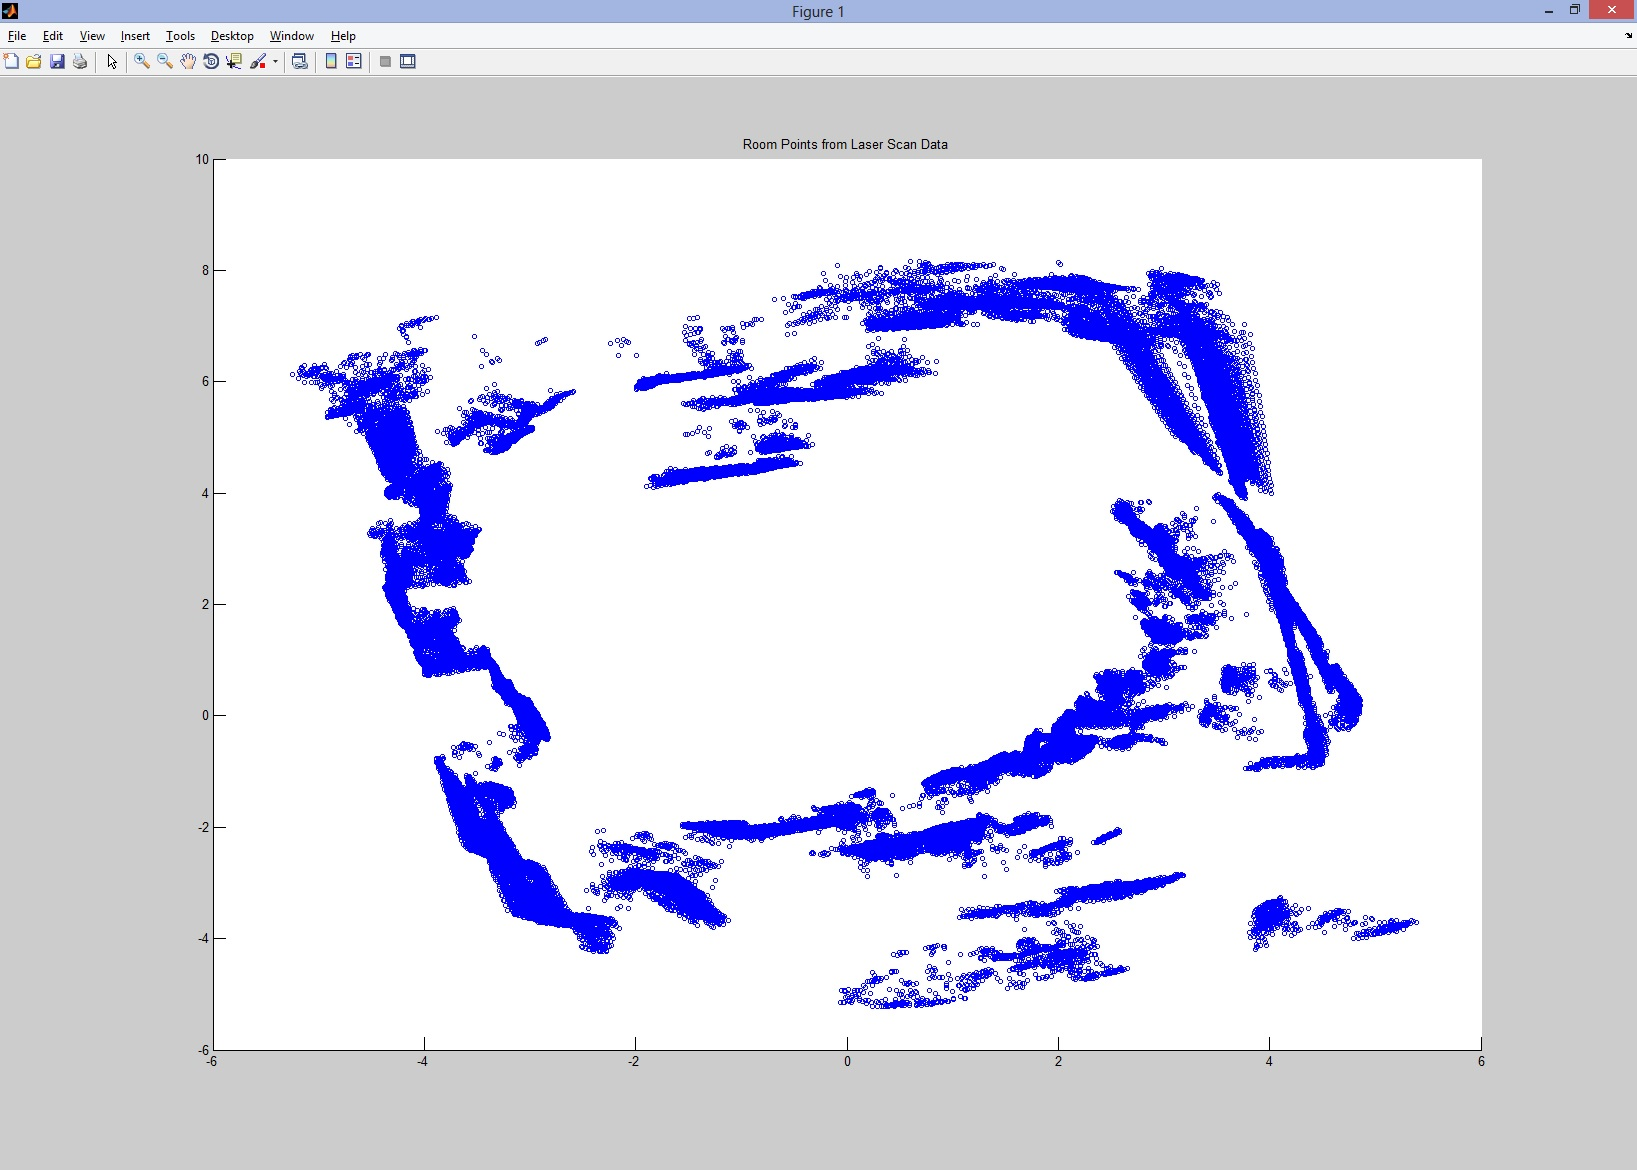
\includegraphics[width=0.8\textwidth]{lab01/lab01_material/part1/me132_tutorial_player/Room.jpg} \end{center} \label{tut1}
\end{figure}

\subsection{Tutorial 2}
When we execute this program we obtain the below image. We can see that the features in both the test and reference image are matched with lines connecting the feature pairs.
\begin{figure}[H]
\begin{center} \includegraphics[height=0.8\textwidth]{lab01/lab01_material/part1/me132_tutorial_camera/capture.png} \end{center} \label{tut2}
\end{figure}

\subsection{Tutorial 3}
We obtain results similar to the above, except that the two images update from a stereo camera and we can see features matched between them. Alternatively, a version named \verb|me132_tutorial_3v2| is available which fixes a reference image with a given file and compares it to the right image from the stereo camera. The output from these are saved in \verb|right_stereo_3D.txt|. The data is saved in the form \verb|[x, y, z, r, g, b]| as .csv file to be plotted by \verb|me132_tutorial_3_plot.m|.\\
The data from the robot demo is saved in \verb|data.txt| and results in the following image:
\begin{figure}[H]
\begin{center} 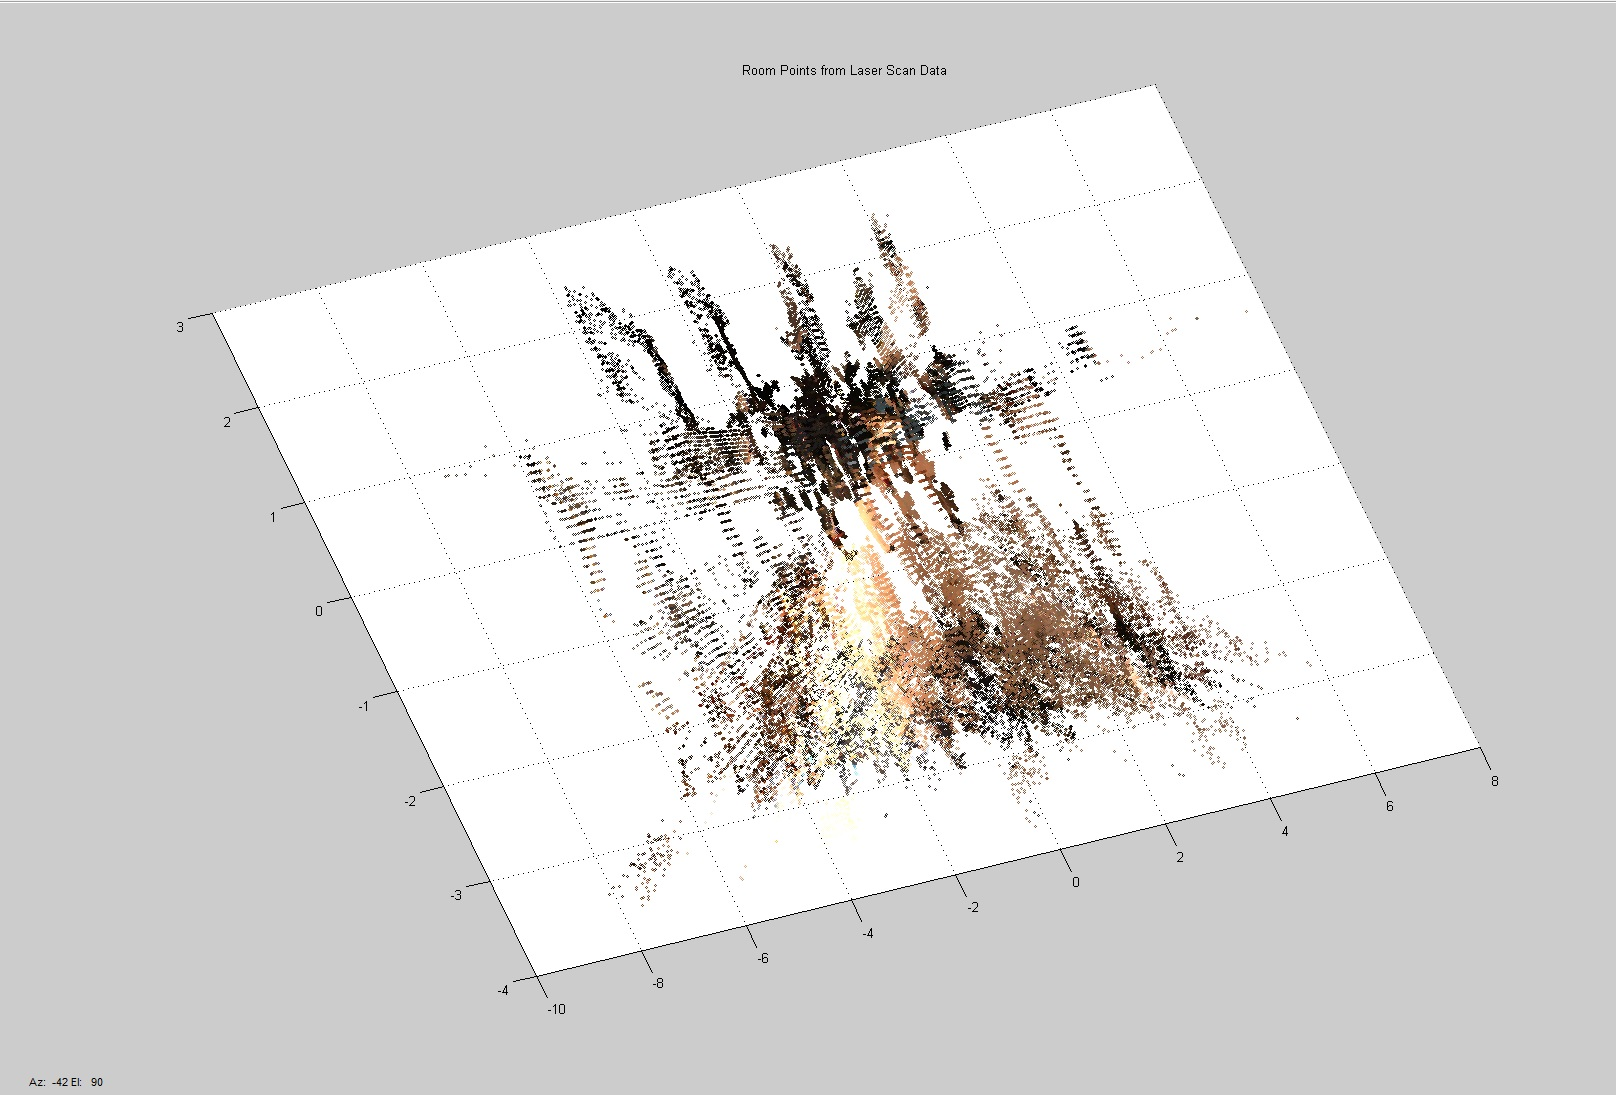
\includegraphics[width=0.8\textwidth]{lab01/lab01_material/part1/me132_tutorial_camera/tutorial3_image.jpg} \end{center} \label{tut3}
\end{figure}

\section{Part 2}

\subsection{Run Time Notes}
All driving code is in \verb|ME132_Lab1.m|. The code is partitioned into cells so that later figures can be run independently once the earlier data is read in properly. The code run time is heavily dependent on the size of the input images. With the full size original example images the SIFT read in portion takes about 2.5 minutes while the histogram generation and feature matching takes approximately 45 minutes on all 3 example images. This is due to the cross image feature matching that requires very large arrays. Scaling the images down can significantly increase run time.
Note: object image 2 and 12 had to be scaled down since \verb|siftWin32.exe| runs out of memory if the images are too large.

\subsection{Output files}
All files are inside the \verb|sift| folder. Images are labeled with the figure letter and a number to indicate the corresponding example or object image. The input object images have a copy in the \verb|object_imgs - scale| folder which are reduced to 600 pixels across.\\
For the feature matching across two images, we plot the features in matching colors. For Figure F, we can see that the homography transform works by comparing the color regions for each feature.

\subsection{Results - Test}

The output from a run on my computer. The homography matrix and the XY coordinates correspond to example images 1-3 in order.
\begin{verbatim}
Time to load images was 1.3258
Finding keypoints... 
3814 keypoints found. 
Finding keypoints... 
8028 keypoints found. 
Finding keypoints... 
3463 keypoints found. 
Finding keypoints... 
679 keypoints found. 
Finding keypoints... 
6344 keypoints found. 
Finding keypoints... 
11258 keypoints found. 
Finding keypoints... 
18117 keypoints found. 
Finding keypoints... 
13159 keypoints found. 
Finding keypoints... 
8236 keypoints found. 
Finding keypoints... 
12894 keypoints found. 
Finding keypoints... 
6240 keypoints found. 
Finding keypoints... 
77262 keypoints found. 
Finding keypoints... 
916 keypoints found. 
Finding keypoints... 
1296 keypoints found. 
Finding keypoints... 
1101 keypoints found. 
Time run sift was 154.6458
Time for figure A 5.7155
Time for figure B 1.2233
Time for figure C 2720.1311

H =  20.5     -6.7    -868.8
     10.1     12.6   -3931.7
      0.0     -0.0       1.0
rowcol = [114.8711, 219.6791]
xyz = [ 42.8741,  81.9976,   0.3733]

H =   6.7     -3.8     275.5
      5.1      3.1   -1033.0
      0.0      0.0       1.0
rowcol = [ 76.8476, 207.0157]
xyz = [ 39.1513, 105.5151,   0.5098]

H =  2.4     -5.5    1433.9
     6.3     -0.2    -795.6
     0.0     -0.0       1.0
rowcol = [134.6543, 321.5502]
xyz = [ 83.0928, 198.4456,   0.6172]
\end{verbatim}

\subsection{Results - Demo}
When running on the example 10 image, we obtain the following homography transform results for the two objects detected (3 and 11) respectively. Note that for speed during the demo, the scaled versions of the object images.
\begin{verbatim}
OBJECT 3:
H = 2.9339   -0.0841 -390.1813
    0.1445    2.8881 -109.2425
    0.0001   -0.0001    1.0000
rowcol = [133.8839,  31.1262]
xyz = [ 71.9144,  16.7180, 0.5380]
OBJECT 11:
H =  2.6    2.0   -1082.6
    -1.9    2.5    -242.0
     0.0    0.0       1.0
rowcol = [220.0172, 259.3230]
xyz = [106.2697, 125.2662, 0.4831]
\end{verbatim}

\end{document}
